% Höfundur/Author: Hákon Örn Árnason - hakona07 AT ru.is
% Viðhaldið af/Maintained by: Hákon Örn Árnason - hakona07 AT ru.is
%%%%%%%%%%%%%%%%%%%%%%%%%%%%%%%%%%%%%%%%%%%%%%%%%%%%%%%%%%%
% Credits to:
% Math template by Hlynur Arnarsson
% How to write text by Andrei Manolescu, Haraldur Auðunsson, Sigurður Ingi Erlingsson, version 050918
% Hákon Valur Haraldsson - figures and tables additions.
%%%%%%%%%%%%%%%%%%%%%%%%%%%%%%%%%%%%%%%%%%%%%%%%%%%%%%%%%%%

\documentclass{scrartcl}
% Skapalón frá Hlyni Arnórssyni
% Physics Version 0.2 - 10.Jan 2020
% ---------- Blaðsíðustillingar ---------- 
\usepackage{geometry}

\geometry{
	paper=letterpaper, %a4paper, % letterpaper lika til
	top=2.5cm, % Top margin
	bottom=1cm, % Bottom margin
	left=2.5cm, % Left margin
	right=2.4cm, % Right margin
	headheight=0.75cm, % Header height
	footskip=1.5cm, % Space from the bottom margin to the baseline of the footer
	headsep=0.75cm, % Space from the top margin to the baseline of the header
	%showframe, % Uncomment to show how the type block is set on the page
}

% ---------- Íslenska ---------- 
\usepackage[T1]{fontenc}
\usepackage[utf8]{inputenc}
%\usepackage[icelandic]{babel} % Setið 'english' í hornklofana ef skýrslan er alfarið á ensku.
\usepackage[english]{babel} % Setið 'english' í hornklofana ef skýrslan er alfarið á ensku.

% ---------- Stærðfræðipakkar frá AMS ---------- 

\usepackage{amsmath, amsfonts, amsthm, amssymb} % Stærðfræðipakkar
\usepackage{braket, nicefrac} % fyrir mengi, brotabrot

% ---------- Fyrir SI Einingar ---------- 
\usepackage{siunitx}

% ---------- Listar/ númeringar ---------- 
\usepackage{enumitem, multicol}

% ---------- Fyrir innsetningu mynda ---------- 
\usepackage{graphicx, float} 
\usepackage{keystroke}
\usepackage{pgfplots}\usepgfplotslibrary{units}
\pgfplotsset{width=10cm,compat=1.9}
\usepackage{caption}
\newcommand{\source}[1]{\caption*{Source: {#1}} }

% ---------- Til að teikna/tekka myndir ---------- 
\usepackage{tikz}
\usepackage{tkz-euclide}
\usetikzlibrary{math}
\usepackage{fourier}
\usetikzlibrary{quotes,angles}
\usepackage{tkz-euclide}
\usetikzlibrary{calc}
\usepackage[siunitx, nooldvoltagedirection]{circuitikz} %%<--- Circuit Diagrams/Rafrása myndir
\usepackage{csquotes}
%%%%%%%%%%%%%%%%%%%%%%%%%% Hyperlink References %%%%%%%%%%%%%%%%%%%%%%%%%%%
\usepackage[colorlinks=true, linkcolor=blue, citecolor=blue, urlcolor=blue, bookmarks=true, breaklinks=true]{hyperref}
\labelformat{equation}{(#1)} %jöfnu fix
\def\equationautorefname#1{}%for autoref, gobble the space
%%%%%%%%%%%%%%%%%%%%%%%%%%
% ---------- Nýtt Matlab viðmót ---------- 
\usepackage{listings}
\usepackage{fancyvrb}

\def\lstbasicfont{\fontfamily{pcr}\selectfont\normalsize}
\definecolor{mygreen}{RGB}{28,172,0} 
\definecolor{mylilas}{RGB}{170,55,241}
\lstset{language=Matlab,%
	basicstyle={\lstbasicfont},
	breaklines=true,%
	morekeywords={matlab2tikz},
	keywordstyle=\color{blue},%
	morekeywords=[2]{1}, keywordstyle=[2]{\color{black}},
	identifierstyle=\color{black},%
	stringstyle=\color{mylilas},
	commentstyle=\color{mygreen},%
	showstringspaces=false, %without this there will be a symbol in the places where there is a space
	numbers=left,%
	numberstyle={\tiny \color{black}},% size of the numbers
	numbersep=5 pt, % this defines how far the numbers are from the text 
	inputencoding=latin1,
	backgroundcolor = \color{gray!3},
	framexleftmargin= -1 mm,
	frame=none,
	rulesepcolor=\color{blue!30},
	extendedchars=true,
	emph={logical},emphstyle=\color{blue},	
	emph={all,equal, minor, on, off, long, short, bank, rat},emphstyle=\color{mylilas},	
}
\renewcommand\lstlistingname{\textsc{Matlab}}%

\usepackage{tcolorbox}
\tcbuselibrary{skins}
% ---------- Hérna vel ég stillingar fyrir ramma sem ég skýri matlabUT
\tcbset{matlabUT/.style={
		enhanced,
		colback=gray!1,
		colframe=gray!30,
		title=Command Window,
		arc=0mm,
		coltitle=black,
		center title, 
		title style={top color=white, bottom color = gray!30},
		grow to left by= -3 mm,
		left= 4 mm,
		grow to right by=0.5mm,
		colupper = gray!70!black
}}

%  ---------- Les inn textaskra sem inniheldur niðurstöður úr Command Window
\newcommand{\CommandWindow}[1]{\begin{tcolorbox}[matlabUT]
		\VerbatimInput{#1}
\end{tcolorbox}}


%%%%%%%%%%%%%%%% Matlab endar %%%%%%%%%%%%%%%%%%%%%%%%%%%%%%%%%%%%%%%%

%%%%% Geogebra  %%%%%%%%%%%%%%%%%%%%%%%%%%%%%%%%%%%%%%%%%%%%%%%%%
% ---------- Nokkur tól í GeoGebru, smíða einnig skurðtólið ---------- 

\newcommand{\Punktur}{% Punktur í GeoGebru
	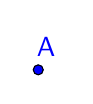
\begin{tikzpicture}[scale = 2]
	\draw
	(0,0) coordinate(A)
	(0.05,0.025) coordinate(pos)
	node[blue, anchor = south] {$\mathsf{A}$}  
	[blue,fill](A) circle(0.85pt); 
	\draw      [color = black](A) circle(0.9pt);
	\end{tikzpicture}
}
\newcommand{\Linustrik}{%  Strik, segment
	
\begin{tikzpicture}[scale = 0.4]
	\draw
	(0,0) coordinate(A)
	(1,0.7) coordinate(B)
	[line width = 1pt, blue](A)--(B);
	\draw[blue, fill](A) circle(4pt);
	\draw[blue, fill](B) circle(4pt);
	\end{tikzpicture}	
}

\newcommand{\Lina}{% bein lína, hægt að framlengja að vild
	
\begin{tikzpicture}[scale = 0.5]
	\draw
	(0,0) coordinate(A)
	(1,0.7) coordinate(B)
	[line width = 1pt, blue](A)--(B);
	\draw[blue, fill](0.25,0.18) circle(3pt);
	\draw[blue, fill](0.74,0.53) circle(3pt);
	\end{tikzpicture}	
}
\newcommand{\Halflina}{% við smíð á hornum
	
\begin{tikzpicture}[scale = 0.4]
	\draw
	(0,0) coordinate(A)
	(1,0.7) coordinate(B)
	[line width = 1pt, blue](A)--(B);
	\draw[blue, fill](A) circle(3pt);
	\draw[blue, fill](0.65,0.45) circle(3pt);
	\end{tikzpicture}	
	
}

\newcommand{\GeoO}{
	\begin{tikzpicture}[rotate=30,transform canvas={scale=0.18},yshift=7mm]
	\def\xrad{0.7}
	\def\yrad{0.58}
	\definecolor{GeogebraLitur}{rgb}{0.6,0.60,100}
	\tikzset{hnutur/.style={shape=circle, line width=0.7mm,color=black, fill=GeogebraLitur, scale=0.8, draw}} % 0.8
	\draw[ color = gray!70!black, line width=1.3mm] (0,0) circle[x radius = \xrad cm, y radius = \yrad cm];
	\def\n{5}
	\foreach \k in {1,...,\n}
	\node at ({360/\n*\k-10}:\xrad cm and \yrad cm)[hnutur] {};
	%	node[pos=1,hnutur]{} ;
	\end{tikzpicture}
}
\newcommand{\Geogebra}{{\color{gray!70!black}\textsf{Ge}\ \GeoO\textsf{Gebra }}}




% ---------- Skrá fyrir myndir ---------- 
\graphicspath{{graphics/}{Graphics/}{./}}
% ---------- Skrá fyrir heimildir ---------- 
% \usepackage[style=ieee]{biblatex}
% \addbibresource{bibliography.bib}
\usepackage{amsmath}

\begin{document}

%% --- Titil síða / Title page --- %%
\begin{titlepage}
	\centering
	
\includegraphics[width=0.8\textwidth]{College_of_Arts_and_Sciences_H_Black.eps}\par\vspace{1cm} %<-- CAS Logo
	{\scshape\LARGE Ohio University \par} 
	\vspace{1cm}
	{\scshape\Large Edwards Accelerator Lab\par} 
	\vspace{1.5cm}
	{\huge\bfseries Tank Opening Report - February 2023\par} 
	\vspace{2cm}
	{\Large\itshape Gregory Leblanc}\par
	\texttt{leblanc at ohio.edu}\par 
	\vspace{0.5cm}
	{\Large\itshape Don Carter}\par
	\texttt{carter at ohio.edu}\par 
	\vfill
	\vfill

% Bottom of the page
	{\large \today\par}
\end{titlepage}

%% --- Titil síða endar / Title page ends --- %%

\section{Reason for Opening} %<--  Inngangur / Introduction

Several performance problems had been noted recently triggering this tank opening.  Excessive Y-steering 
was required in order to get the beam through the swinger, and extremely poor transmission was noted with the 
swinger at 0 degrees.  We also noted instability in the HE tube current, so we wanted to check the HE tube 
resistors. More than the expected amount of voltage on the tube entrance lens was required.  Not enough to 
indicate a significant problem, but enough to warrant inspection.  We had also experienced several sparks
while conditioning for operation at maximum terminal voltage (>4.5MV), which is another cause for resistor
inspection.  The straw that broke the camel's back was the chain stretch alarm occuring on several runs.  
The alarm seemed to clear after allowing sufficient time for the accelerator to cool.  We had also 
noted abnormally high tank temperatures during operation.


\section{Summary of work} 

\subsection{Tank Opening}

\subsubsection{2023-02-09 Thursday}
\begin{itemize}
    \item Pumped SF6 from Tandem into gas storage tank. FIXME: Insert final storage conditions here.
    \item Tank was left open to air, but access hatch was left closed.
\end{itemize}

\subsubsection{2023-02-10 Friday}
\begin{itemize}
    \item Don was out today.  Decided to delay permit required confined space and access hatch opening until Monday.
	\item Began work on SF6 recirculator.  Pressure vessel for blower (PIG) was found to be dirty and full of small brass 
	shavings.  Logbook entries from previous tank openings indicate that these are probably from the pressure relief 
	valve.  Inside of the pig was scrubbed using soapy water and a nylon brush attachement on a drill.  Visisted 
	machine shop to discuss PRV issue.  Removed PRV and cleaned for delivery to the shop next week.  Removed blower and
	blower motor support structure, and started cleaning.  A significant quantity of foamed grease was noted below the back
	end of the blower, probably from the bearings on that end of the blower.  
	Unable to open valve 10, possibly excessive pressure difference across
	the valve.  Will investigate further next week.
\end{itemize}

\subsubsection{2023-02-13 Monday}
\begin{itemize}
	\item Performed permit required confined space entry with Don.  Installed platforms in bottom of tank and lights.  
	Converted permit-required confined space to non-permit required space.
	\item Delivered PRV to machine shop for inspection.  Visited machine
	shop to disassemble and inspect valve.  
	\item Measured clearance from floating motor platforms to column base, with motors both on and off.  Chain 3 (FIXME?)
	is very close to the chain stretch alarm switch.  Inspected spare 
	switches to get an idea of switch travel.  Calculated thermal chain 
	stretch assuming 10(FIXME) degrees C rise and the chain made entirely
	of nylon.
	\item Measured column resistance hoop-to-hoop with Kate.  No excessive 
	values noted, but meter readings on the tester fluctuated significantly.
	Need to recheck later and measure across each plane.
\end{itemize}

\subsubsection{2023-02-14 Tuesday}
\begin{itemize}
    \item Discussed valve with Doug at the machine shop.
    \item Investigated cooling water for tank.  Found that there was a
    solenoid located in the pit.  Reviwed drawings with Don, and found 
	some interlocks with the old belt drive.  Decided that it was th
	day and that we should review in the morning.
\end{itemize}

\subsubsection{2023-02-15 Wednesday}
\begin{itemize}
    \item Don found some drawings that were updated at the time of the 
    Pelletron upgrade, and we determined that the solenoid was linked to
	the tank door switch, and powered by one of the circuit breakers in
	the control room.  Found that the door switch was no longer sealed
	against water intrusion, and that it was stuck in the closed position.
	Don cleaned and repaired the switch, then we tested operation.  \par
	Also found that the circuit breaker in the control room was the one
	that we found already in the "off" position when we performed the 
	tank entry procedure.  Since the switch wasn't sealed, we believe
	that the switch shorted to ground during the floor causing the breaker
	to trip.  This would have left us without any cooling water circulating
	inside of the tank, but wouldn't have affected anything else.  Our 
	belief is that we haven't had cooling water since the flood last July.
	\item Trained grad students (Mike, Joseph, and Nisha) on cleaning the
	cooling coils inside the tank.  Left them the shop vac, long hoses,
	cleaning brushes, and microfiber cloths.
	\item Re-measured the column resistors with Kate, this time across 
	each plane instead of from hoop to hoop.  Removed one of the columnn
	resistors to measure without all of the various connection points
	involved when the resistor assembly is mounted to the column.  Found
	that the resistance reading was very stable when measured this way.
	\item Added additional tape to the LE carpet so that I could stand
	and use the measurement tool to check the springs connecting the
	resistors to the acceleration planes.  Tested using the tool, and
	found that resistance values were much less stable when testing 
	with the megger.  Removed a couple of resistors for a closer inspection
    and found that the resistance values were very stable.  Probably 
	no problems here, but will double-check next week to insure no open-
	circuits are present, indicating missing springs.  The unstable readings
	are probably just from the surface corrosion on the springs and the 
	relatively low testing voltage (1kV).  
	\item Don looked up the drawings showing which planes are inclined 
	which direction.  Will review this data against David's spreadsheet
	and against our resistance measurements.  
\end{itemize}

\subsubsection{2023-02-16 Thursday and 17 Friday}
\begin{itemize}
	\item Greg out.  Will ask others for prose here.
\end{itemize}

\subsubsection{2023-02-20 Monday}
\begin{itemize}
	\item Noon start today.  Drained oil from SF6 blower.  Oil was quite
	dark compared with the clear blue color of new oil.  Refilled blower
	with 175 ml of oil, but no oil visible in drain port.  Reviwed docs, 
	found that I had used the wrong hole. Drained oil to the correct 
	level.  
	\item Counted acceleration plane resistors on drawings.  Drawings 
	seem to show 49 UP planes and 47 DOWN planes.  Assuming some 
	mistake somewhere, and the correct numbers are 48 each way, we have 
	a deviation of less than 1\%.  
\end{itemize}

\subsubsection{2023-02-21 Tuesday}
\begin{itemize}
	\item Started Lectro-Dryer to regenerate desicant system.  System ran 
	and came up to temperature, then failed and shut down.  Alert levels 
	were triggered on VESDA system.  Inspection revealed the fuses in
	the control panel had failed and gotten hot enough to melt insulation
	on the wires and the solder out of the end of the fuses.
	\item Prose here.
\end{itemize}

\subsubsection{2023-02-22 Wednesday}
\begin{itemize}
	\item More blower work with Don and Doug.  Installed a pressure gauge
	on the output of the blower. Found 0 PSI and 2.4 A draw with the outlet
	valve open.  Approximately 6.5 PSI and 3.3 A draw (3.0 FLA on motor
	nameplate) with outlet valve completely closed.  \par
	Pressure relief valve (PRV) was modified to lock the ring against the
	casting, instead of in the factory position where it seemed to
	interfere with valve seating (factory calls this "simmer").
	\item Changed pipe dope on all 3 filter housings.  
	\item Repaired burnt wiring in Lectro-Dryer control panel.  
	\item Worked on PIG install.  Nothing was quite at the right height
	so the overhead crane was used to help get the alignment pins installed.
	Jack-bolt holes are partially stripped, and the jack bolts aren't long
	enough to pull everything together.  Will resume tomorrow.
\end{itemize}

\subsubsection{2023-02-23 Thursday}
\begin{itemize}
	\item Opened PIG and lubed chain coupling with LPS-1.  Wiped excess 
	while motor was running.
	\item Reinstalled PIG.  Still difficult, but eventually got
	everything to line up and retaining pins dropped in without problem.
	\item Work on chains.  Counted 154 links on chain 2, and worked with Don
	to try to remove a link for an hour or two before lunch, then decided
	we all needed a break.  After lunch developed a new link removal 
	procedure, and successfully shorted all 3 chains by 1 link.  All 3
	chains still have at least one more location where there is a 
	"double master link" and can be shortened further.
\end{itemize}

\subsubsection{2023-02-24 Friday}
\begin{itemize}
	\item Measured chain stretch on all 3 chains.
	\begin{center}
		\def\arraystretch{1.3}
		\begin{tabular}{ |c|c|c| }
			\hline
			Chain & Static & Dynamic \\
			\hline
			Chain 1 & 2 \(\frac{3}{8}\)" & 2" \\
			Chain 2 & 2 \(\frac{1}{2}\)" & 2 \(\frac{1}{8}\)" \\
			Chain 3 & 1 \(\frac{1}{2}\)" & 1 \(\frac{1}{8}\)" \\
			\hline
		\end{tabular}
	\end{center}
	\item Cleaned all chains.  Initial cleaning with microfiber cleaning
	cloth produced no change.  Kimwipes + IPA removed the "dull" finish
	on all chain links are resored them to bright shiny condition like 
	a new chain.  No attempt was made to clean the nylon portions of the
	links, but they also did not appear to be very dirty.
	\item Reassembled all column hardware that was removed to make room
	for chain link removal.  
\end{itemize}

\subsubsection{2023-02-27 Monday}
\begin{itemize}
	\item First day of extended shutdown.  
	\item Disconnected tube entrance lens and remeasured LE "low 
	value" resistors entrance lens.  See attached table. 
	FIXME: add link to table.
	\item Removed carpet from inside of tank, and cleaned up Gorilla
	Tape residue with acetone.  Extra cleanup here is probably a good
	tradeoff for additional safety while inspecting resistors.
	\item Re-checked and torque marked all \(\frac{5}{16}\)" bolts on 
	motors.  All bolts were marked with yellow paint pen.  Found 1 loose
	bolt that was missed on the first torque check.
	\item Ran chains and powersupplies in air.  Ran charging voltage
	high enough to see that current was balanced on all 3 chains. 
	GVM did not indicate any voltage (motor probably not running).
	\item Initiated confined space permit and removed flooring.
	\item Roughed accelerator and left at vacuum overnight.  Accelerator
	tubes are built to withstand external pressure, so they must always be
	at vacuum when the tank is at vacuum.  Original wisdom was to only
	rough the tank while attended, so that it could be vented in the event
	of a vacuum failure in the accelerator tubes.  Need more thought on
	this.
\end{itemize}

\subsection{2023-02-28 Tuesday}
\begin{itemize}
	\item Equalized pressure from storage into accelerator and started
	leak checking.  Found a large SF6 leak in the vicinity of the PIG, 
	so SF6 was pumped back into storage and acccelerator vented to air
	overnight.
\end{itemize}

\subsection{2023-03-01 Wednesday}
\begin{itemize}
	\item Cleaned and reinstalled tank entry hatch seals. Everything
	here looked good.
	\item Opened PIG and found on section of the Lenape seal that looked
	dry vacuum grease and was out of place compared with seals elsewhere.
	Removed seals, cleaned, and reinstalled everything with extra care.
	\item Pumped gas back into accelerator.  No leaks initially detected.
\end{itemize}

\end{document}
